% Options for packages loaded elsewhere
\PassOptionsToPackage{unicode}{hyperref}
\PassOptionsToPackage{hyphens}{url}
%
\documentclass[
]{article}
\usepackage{lmodern}
\usepackage{amssymb,amsmath}
\usepackage{ifxetex,ifluatex}
\ifnum 0\ifxetex 1\fi\ifluatex 1\fi=0 % if pdftex
  \usepackage[T1]{fontenc}
  \usepackage[utf8]{inputenc}
  \usepackage{textcomp} % provide euro and other symbols
\else % if luatex or xetex
  \usepackage{unicode-math}
  \defaultfontfeatures{Scale=MatchLowercase}
  \defaultfontfeatures[\rmfamily]{Ligatures=TeX,Scale=1}
\fi
% Use upquote if available, for straight quotes in verbatim environments
\IfFileExists{upquote.sty}{\usepackage{upquote}}{}
\IfFileExists{microtype.sty}{% use microtype if available
  \usepackage[]{microtype}
  \UseMicrotypeSet[protrusion]{basicmath} % disable protrusion for tt fonts
}{}
\makeatletter
\@ifundefined{KOMAClassName}{% if non-KOMA class
  \IfFileExists{parskip.sty}{%
    \usepackage{parskip}
  }{% else
    \setlength{\parindent}{0pt}
    \setlength{\parskip}{6pt plus 2pt minus 1pt}}
}{% if KOMA class
  \KOMAoptions{parskip=half}}
\makeatother
\usepackage{xcolor}
\IfFileExists{xurl.sty}{\usepackage{xurl}}{} % add URL line breaks if available
\IfFileExists{bookmark.sty}{\usepackage{bookmark}}{\usepackage{hyperref}}
\hypersetup{
  pdftitle={Tahoe City 3/1/21},
  pdfauthor={Nick Framsted},
  hidelinks,
  pdfcreator={LaTeX via pandoc}}
\urlstyle{same} % disable monospaced font for URLs
\usepackage[margin=1in]{geometry}
\usepackage{graphicx,grffile}
\makeatletter
\def\maxwidth{\ifdim\Gin@nat@width>\linewidth\linewidth\else\Gin@nat@width\fi}
\def\maxheight{\ifdim\Gin@nat@height>\textheight\textheight\else\Gin@nat@height\fi}
\makeatother
% Scale images if necessary, so that they will not overflow the page
% margins by default, and it is still possible to overwrite the defaults
% using explicit options in \includegraphics[width, height, ...]{}
\setkeys{Gin}{width=\maxwidth,height=\maxheight,keepaspectratio}
% Set default figure placement to htbp
\makeatletter
\def\fps@figure{htbp}
\makeatother
\setlength{\emergencystretch}{3em} % prevent overfull lines
\providecommand{\tightlist}{%
  \setlength{\itemsep}{0pt}\setlength{\parskip}{0pt}}
\setcounter{secnumdepth}{-\maxdimen} % remove section numbering

\title{Tahoe City 3/1/21}
\author{Nick Framsted}
\date{3/6/2021}

\begin{document}
\maketitle

\hypertarget{plotting-do-and-temp-in-chambers}{%
\section{Plotting DO and temp in
chambers}\label{plotting-do-and-temp-in-chambers}}

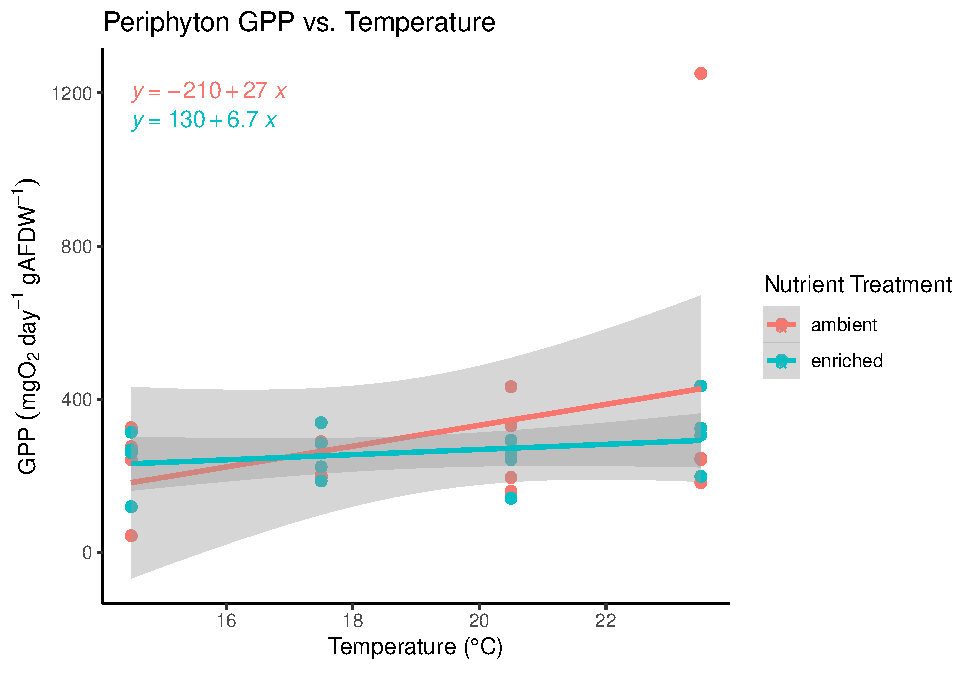
\includegraphics{210301_tahoe_city_inc_files/figure-latex/unnamed-chunk-2-1.pdf}
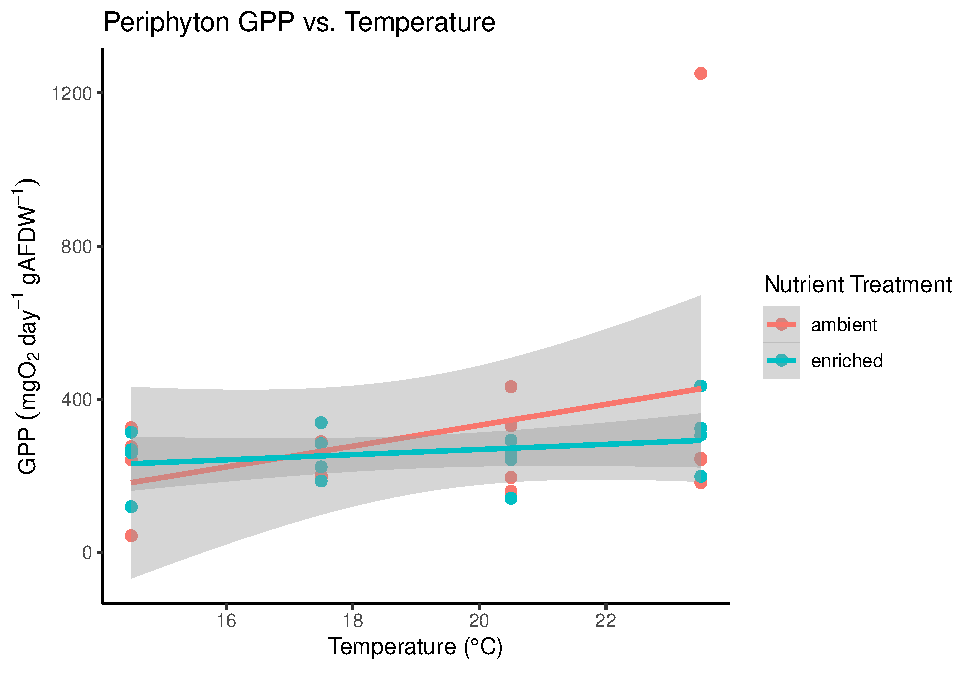
\includegraphics{210301_tahoe_city_inc_files/figure-latex/unnamed-chunk-2-2.pdf}

The weird changes in temperature that cause shifts in DO during the
respiration period of the incubation are due to artificial changes in
temperature measured in the waterbaths, but this does not reflect the
temperatures on the inside of the chambers. This is because the oxygen
concentrations measured in the chambers are incongruous with the
temperature measurements in the waterbaths. The chambers tend to
heat/cool at half the rate as the waterbaths, so temperatures are much
more stable in them compared to the outside water bath. This fact led to
errors in our oxygen measurements.

Possible remedies: 1) Drill holes in 4 unused chambers (1 for each
tank), fill with water at same temperature as tahoe water, and place
temp sensor from presens instrument in each one.

\begin{enumerate}
\def\labelenumi{\arabic{enumi})}
\setcounter{enumi}{1}
\item
  Place a Hobo logger in 4 unused chambers and post-process DO data from
  instrument using Hobo temperature data. This involves intercalibrating
  all temp sensors and adjusting DO data using the Hobo temp Data.
\item
  Splice together segements of respiration signals and remove areas of
  weird data caused by spurious temperature measurements.
\end{enumerate}

\end{document}
